\documentclass{uebblatt}
\usepackage{wrapfig}

\newcommand{\http}{http:/\kern-.2em/\kern-0.03em}

\begin{document}

\maketitle{0}{}

%\vspace{-1em}
%\begin{tiny}
%Eine \emph{Ordinalzahl} stellt einen \emph{Ordnungstyp} dar, d.\,h. eine
%wohlgeordnete Menge. In Mengenlehre kann man eine Ordinalzahl schick als Menge
%ihrer Vorgänger definieren:
%\begin{align*}
%  0 \defeq \emptyset \qquad
%  1 \defeq \{ 0 \} \qquad
%  2 \defeq \{ 0, 1 \} \qquad \\
%  \omega \defeq \{ 0,1,2, \ldots \} \qquad
%  \omega + 1 \defeq \{ 0,1,2, \ldots \} \cup \{\omega\}
%\end{align*}
%Stellen zwei Ordinalzahlen Ordnungstypen~$K$ und~$L$ dar, so definieren wir
%ihre Summe als Repräsentant von~$K \amalg L$ (wobei die Elemente aus~$K$ als
%kleiner als die von~$L$ angesehen werden) und ihr Produkt als Repräsentant
%von~$K \times L$ (mit der lexikografischen Ordnung, wobei die~$L$-Komponente
%als signifikanter angesehen wird). Jede Ordinalzahl ist
%entweder Null, ein direkter Nachfolger einer Ordinalzahl oder sonst eine
%\emph{Limeszahl}. Es gilt das Prinzip der \emph{transfiniten Induktion}:
%Sei~$P(\alpha)$ eine von einer Ordinalzahl abhängige Aussage. Wenn für jede
%Ordinalzahl~$\alpha$ aus der Gültigkeit von $P(\beta)$ für alle~$\beta <
%\alpha$ schon folgt, dass~$P(\alpha)$ gilt, so gilt~$P$ für alle
%Ordinalzahlen.\par
%\end{tiny}
%% Eine Partialordnung heißt genau dann \emph{wohlgeordnet}, wenn ...

\begin{center}
  \begin{minipage}{0.55\textwidth}
    \href{http://naturelovesmath-en.blogspot.de/2012/07/infinity-and-transfinite-numbers.html}{
      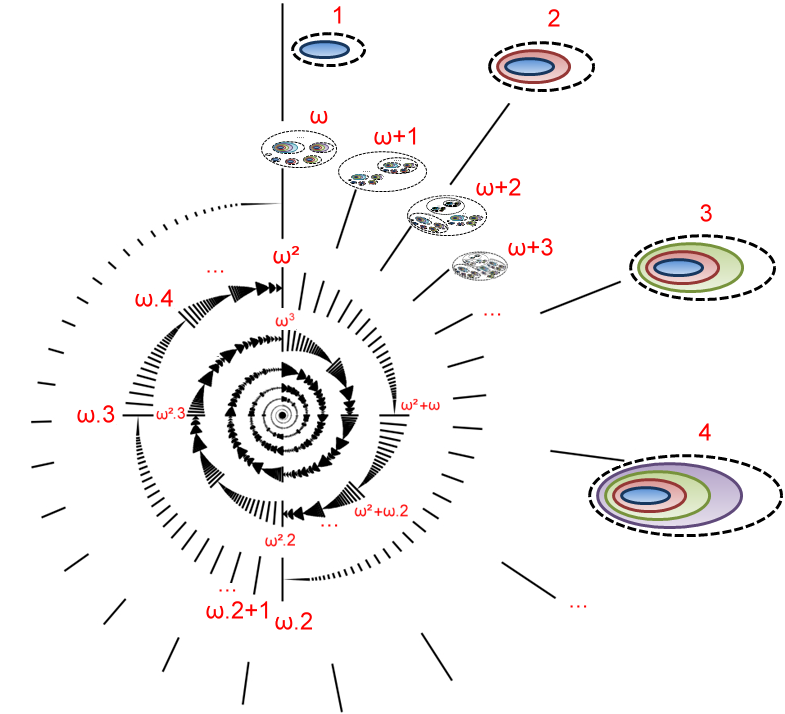
\includegraphics[scale=0.4]{images/ordinal-numbers}
    }
  \end{minipage}
  \qquad
  \begin{minipage}{0.30\textwidth}
    % http://markhkim.com/2013/10/killing-the-hydra/
    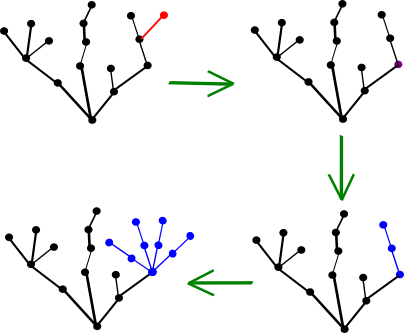
\includegraphics[scale=0.5]{images/hydra}
  \end{minipage}
\end{center}

\begin{aufgabe}{Einbettungen in die rationalen Zahlen}
Sei~$\alpha$ eine \emph{abzählbare Ordinalzahl}, d.\,h. sei die Menge~$M \defeq
\{ \beta \,|\, \beta < \alpha \}$ abzählbar. Bette~$M$ monoton in die
rationalen Zahlen ein! Wie sieht das konkret bei~$\alpha = \omega$, $\alpha =
\omega \cdot 2$ und~$\alpha = \omega^2$ aus?
\end{aufgabe}

\begin{aufgabe}{Herkules vs. Hydra}
Immer, wenn Herkules einen Kopf der Hydra abtrennt, passiert folgendes: Der
Teil der Hydra ab dem jeweiligen Mutterkopf vervielfältigt sich eine gewisse
endliche Anzahl von Malen (siehe Skizze). Es wächst nur dann nichts nach, wenn
der abgetrennte Kopf direkt an der Wurzel lebte. Kannst du Herkules helfen,
diesen ungleichen Kampf zu bestehen?
\end{aufgabe}

\begin{aufgabe}{Freiheit aller Vektorräume}
Sei~$V$ ein Vektorraum. Nach dem Wohlordnungssatz steht~$V$ in Bijektion zu der
Menge aller Vorgänger einer gewissen Ordinalzahl~$\alpha$. Zeige, dass die
Menge derjenigen Vektoren, die nicht im Spann ihrer Vorgänger liegen, eine
Basis von~$V$ ist.
\end{aufgabe}

%\begin{aufgabe}{Links- und Rechtskürzbarkeit}
%Genau eine der folgenden Rechenregeln für Ordinalzahlen ist korrekt. Welche?
%\begin{multicols}{2}
%\begin{enumerate}
%\item Aus~$\alpha + \beta = \alpha + \gamma$ folgt~$\beta = \gamma$.
%\item Aus~$\beta + \alpha = \gamma + \alpha$ folgt~$\beta = \gamma$.
%\end{enumerate}
%\end{multicols}
%\end{aufgabe}

\vfill
\begin{center}
  \rotatebox{90}{\tiny\sffamily \http spikedmath.com/392.html}
  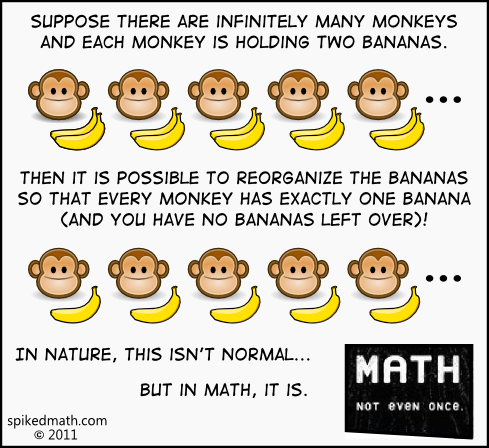
\includegraphics[height=3.7cm]{images/math-not-even-once}
  \qquad
  \rotatebox{90}{\tiny\sffamily \http xkcd.com/982/}
  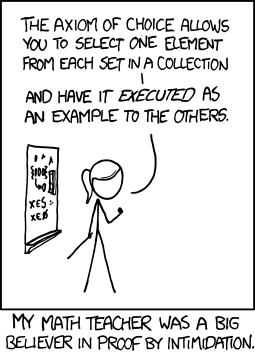
\includegraphics[height=3.7cm]{images/axiom-of-choice}
  \qquad
  \rotatebox{90}{\tiny\sffamily \http spikedmath.com/198.html}
  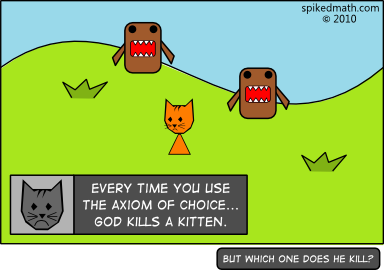
\includegraphics[height=3.7cm]{images/please-think-of-the-kittens}
\end{center}

\end{document}

http://math.stackexchange.com/questions/303704/examples-of-transfinite-induction
http://www.tricki.org/article/Transfinite_induction
http://mathoverflow.net/questions/18357/examples-of-inductive-proofs-that-can-be-generalized-by-transfinite-induction
